\section{Fuel Cycle Simulators}
\subsection{What and Why?}
% ---------------------------------------------- %
% Fuel Cycle Simulators Track Flows of Nuclear Material
\begin{frame}{Fuel Cycle Simulators Track Flows of Nuclear Material}
\begin{columns}
    \column{0.45\textwidth}
    \begin{itemize}
        \item System-scale tool to model nuclear material flow between facilities
        \item Can be as simple as an Excel spreadsheet
        \item Most common usage is transition studies
        \item Should be able to inform non-technical as well as technical decision-makers
    \end{itemize}
    \column{0.55\textwidth}
        \begin{figure}[h]
            \centering
            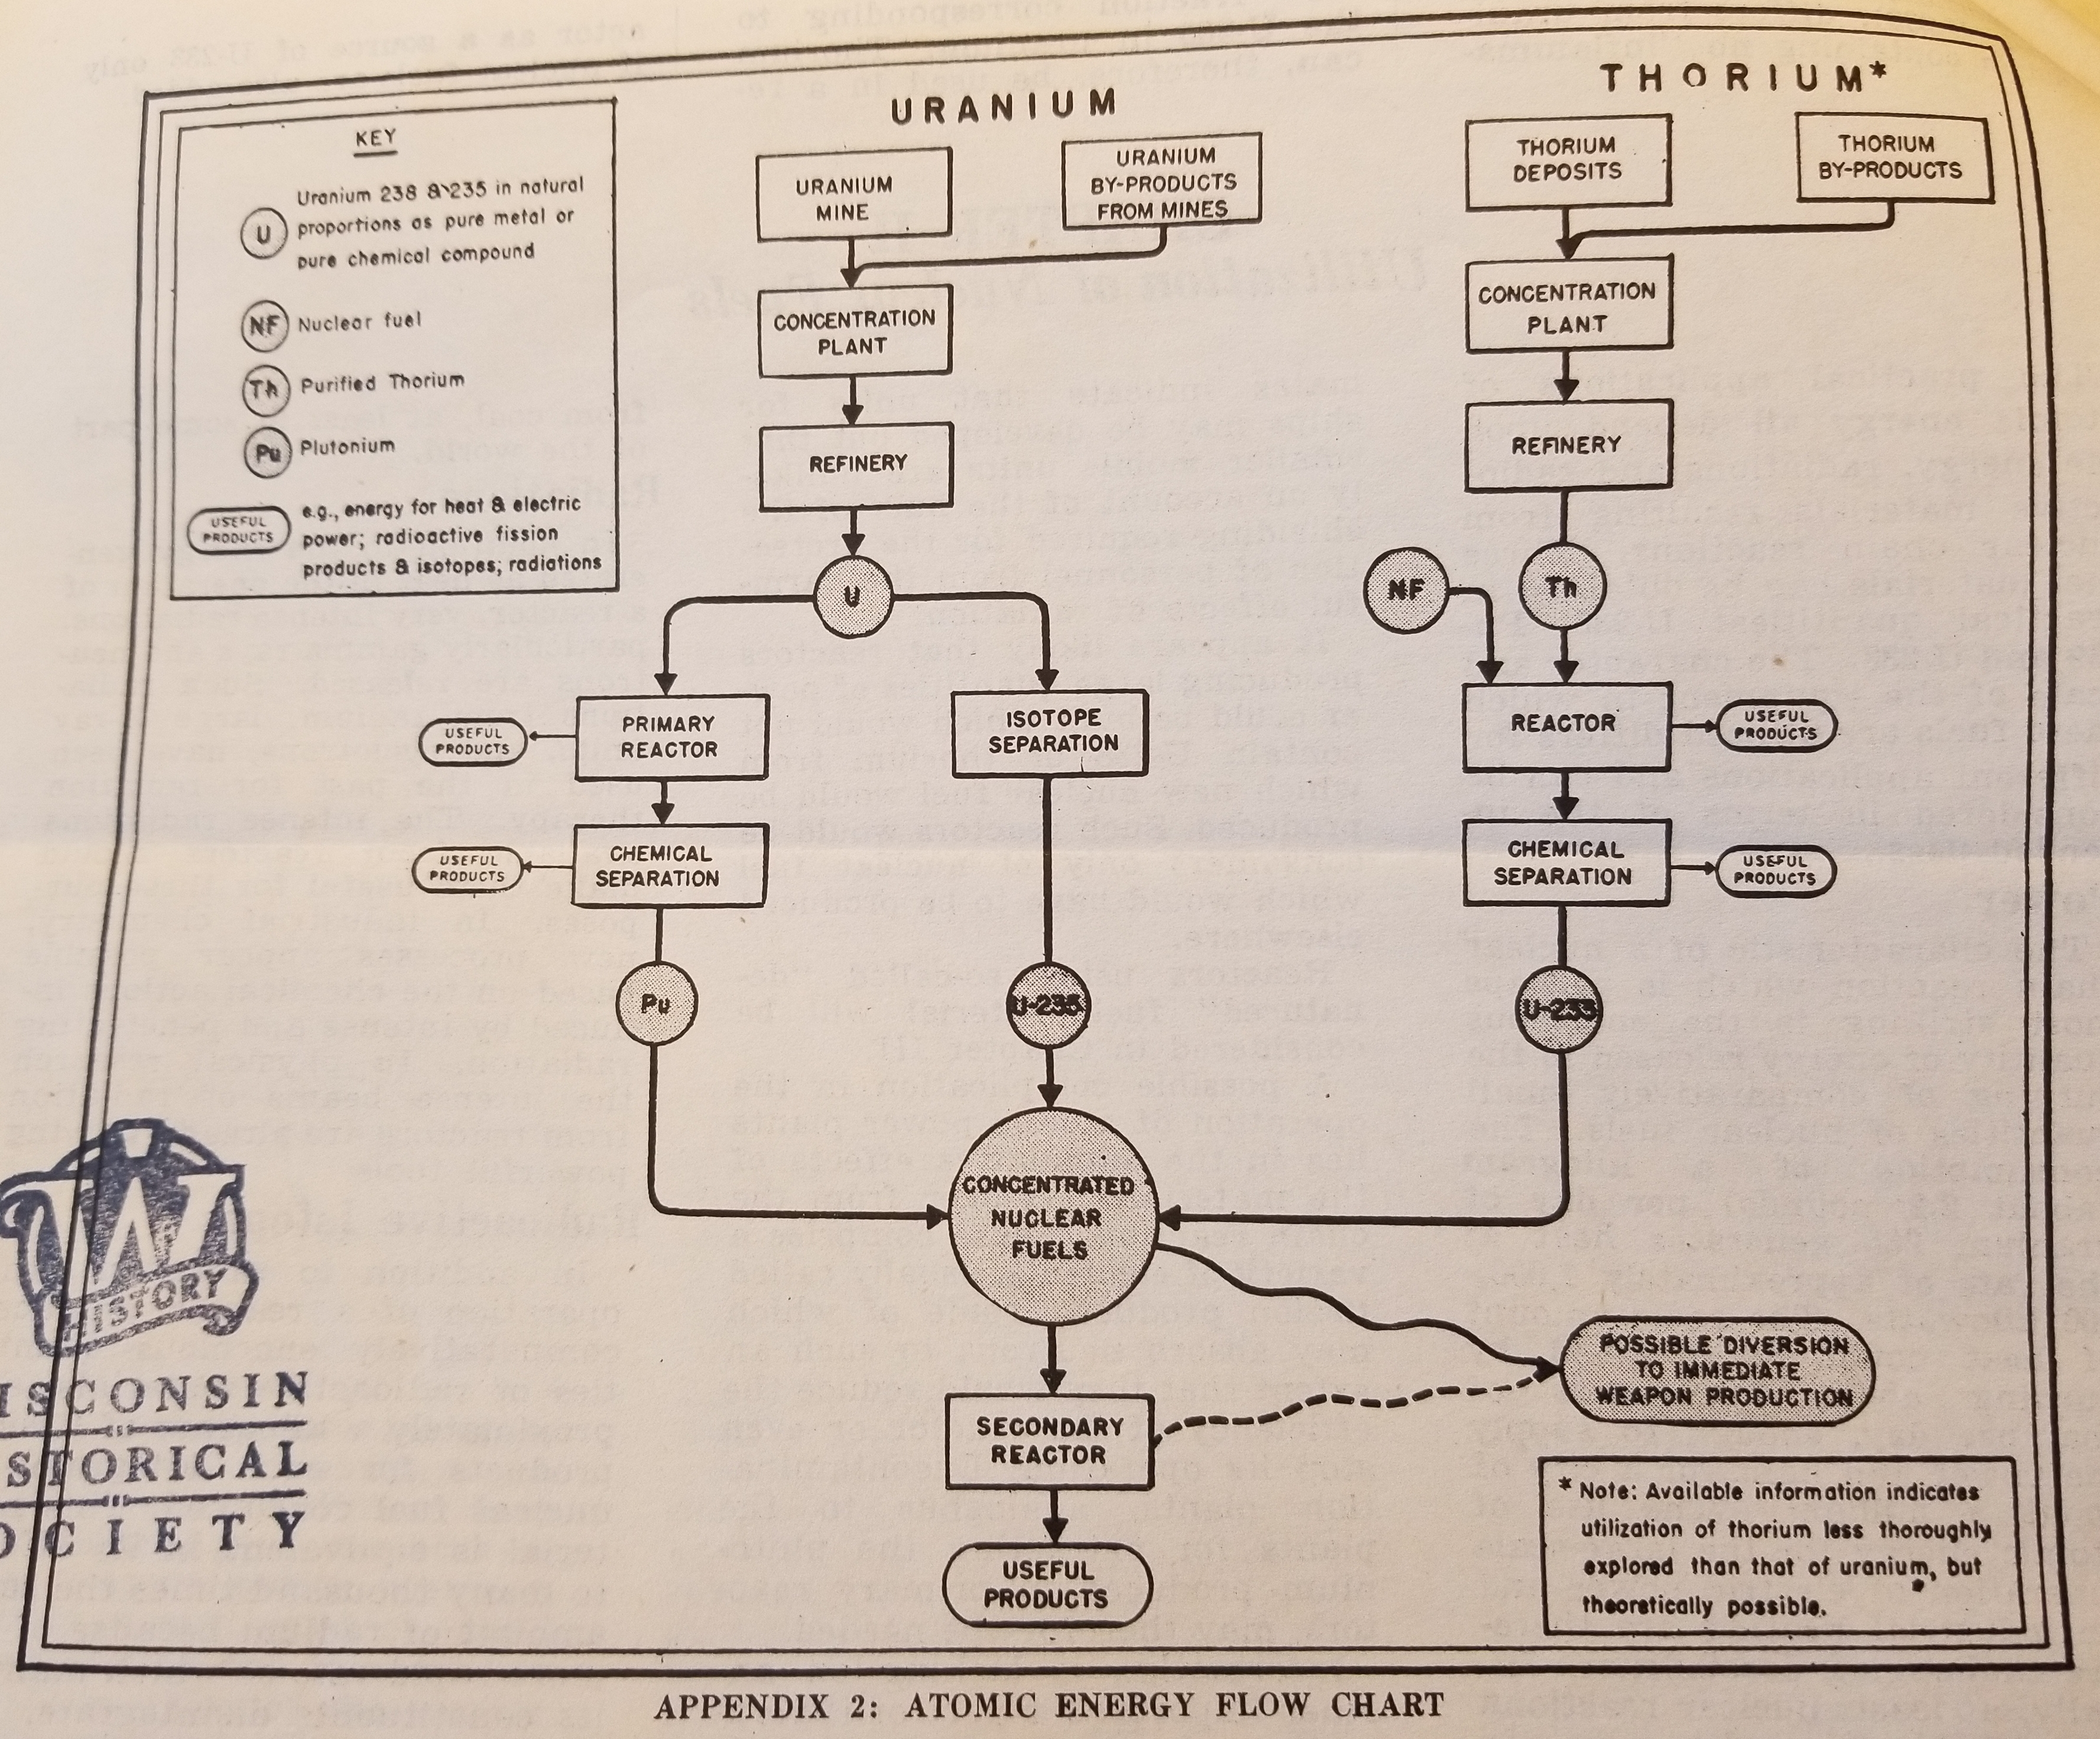
\includegraphics[width=\linewidth]{images/very-old-fuel-cycle1.jpg}
            \caption{U.N. Report, Scientific and Technical Aspects of the Control of Atomic Energy, 1946 \cite{noauthor_scientific_1946}}
            \label{fig:old-fc-diagram}
        \end{figure}
\end{columns}
\end{frame}
% ---------------------------------------------- %

% ---------------------------------------------- %
% Cyclus
\begin{frame}{Transition Studies Require Dynamic (Time-Dependent)\\Capabilities}
    \begin{figure}
        \centering
        \includegraphics[width=\linewidth]{images/Cyclus.png}
        \caption{Classic usage of a fuel cycle simulator includes designing a timeline of new facilities and retirements to transition to a new fuel cycle}
        \label{fig:ABR}
    \end{figure}
\end{frame}
% ---------------------------------------------- %


\subsection{Existing Fuel Cycle Simulators}
% ---------------------------------------------- %
% Cyclus
\begin{frame}{An Incomplete List of Fuel Cycle Simulators}
    \begin{table}[]
    \centering
    %\caption{Fuel Cycle Simulation Tools}
    \small
    \begin{tabular}{|p{2.4cm}|p{2.2cm}|p{2.cm}|p{1.cm}|p{1.3cm}|p{.7cm}|}
        \hline Tool & Developer & Access & Dynam/ \newline Static & Update? & First \newline Pub \\ \hline
        CAFCA \cite{guerin_impact_2009} & MIT & Licensed (f) & D &  Dormant & 2004 \\ %updated?? Discrete
        CLASS \cite{mouginot_core_2014} & France & Open-source & D & Yes & 2013 \\ %Core Library for Advanced Scenario Simulation, Discrete
        COSI \cite{meyer_new_2009},\cite{boucher_cosi:_2006} & CEA & Proprietary & D & Yes & 1991 \\
        \Cyclus \cite{huff_fundamental_2016} & UW--Madison & Open-source & D & Yes & 2011\\ %Discrete
        DANESS \cite{van_den_durpel_daness_2003} & Nuclear21 & Proprietary & D &Yes & 2003 \\
        DESAE \cite{andrianova_desae_2008} & IAEA INPRO & Unknown & D & D & 2006 \\
        DYMOND \cite{moisseytsev_dymond_2001} & ANL & Proprietary & D & Yes &2001 \\
        FUTURE \cite{kim_development_2013} & Korea & Unknown & D & Yes & 2013 \\
        MAKAL \cite{shay_epa_2006} & IEA & Proprietary & D & Yes & 1970s \\
        NFCSim \cite{schneider_nfcsim:_2005} & LANL & Proprietary & D &  No & 2005 \\ %discrete
        NFCSS \cite{noauthor_nuclear_2007} & IAEA & Open GUI & S & Yes & 1996 \\ %Fleet-based
        ORION \cite {worrall_scenario_2007} & ORNL/UKNNL & Proprietary & D & Yes & 2007 \\ %Discrete
        ROADMAP\cite{noauthor_iaea_2018} & IAEA & Unknown & U &  Yes & 2018 \\ %discrete unknown
        SITON \cite{brolly_physical_2017} & Hungary & Unknown & D & Yes & 2017\\ %Discrete
        VISION \cite{jacobson_vision_2009} & INL & Licensed (f) & D & Yes & 2006 \\
        VEGAS \cite{schneider_vegas:_2016} & UT--Austin & Licensed (f) & D & Uknown & 2017 \\   \hline %preconditioner Fleet-based
    \end{tabular}
    \label{tab:FCS}
\end{table}
\end{frame}
% ---------------------------------------------- %

\subsection{Why did UW--Madison create a fuel cycle simulator?}
% ---------------------------------------------- %
% Why another fuel cycle simulator?
\begin{frame}{Why another fuel cycle simulator?}
\begin{columns}
    \column{0.55\textwidth}
    Gaps were noted in fuel cycle simulation capabilities during the Global Nuclear Energy Partnership (GNEP) push of the late 2000s
    \begin{itemize}
        \item Proprietary tools
        \item Mostly focused on reactor simulations
        \item Limited or on ability to novel designs
        \item Static systems
    \end{itemize}
    \column{0.35\textwidth}
    \begin{block}{GNEP in a few words}
        \footnotesize
        \alert{GNEP} began in 2006 as a US-lead effort to expand nuclear energy domestically \& internationally to:
        \begin{itemize}
            \item Reduce usage on fossil fuels/promote clean energy
            \item Encourage proliferation- resistant designs
            \item Assert US dominance as global supplier
        \end{itemize}
        US effort killed by Obama admin amid the Great Recession, international effort replaced by IFNEC
    \end{block}
\end{columns}
\end{frame}
% ---------------------------------------------- %
